% Defense presentation — draft skeleton, to be filled in.
% Build:  cd presentation && tectonic -X compile main.tex
% Figures: use the PDFs in ../figures/, e.g. 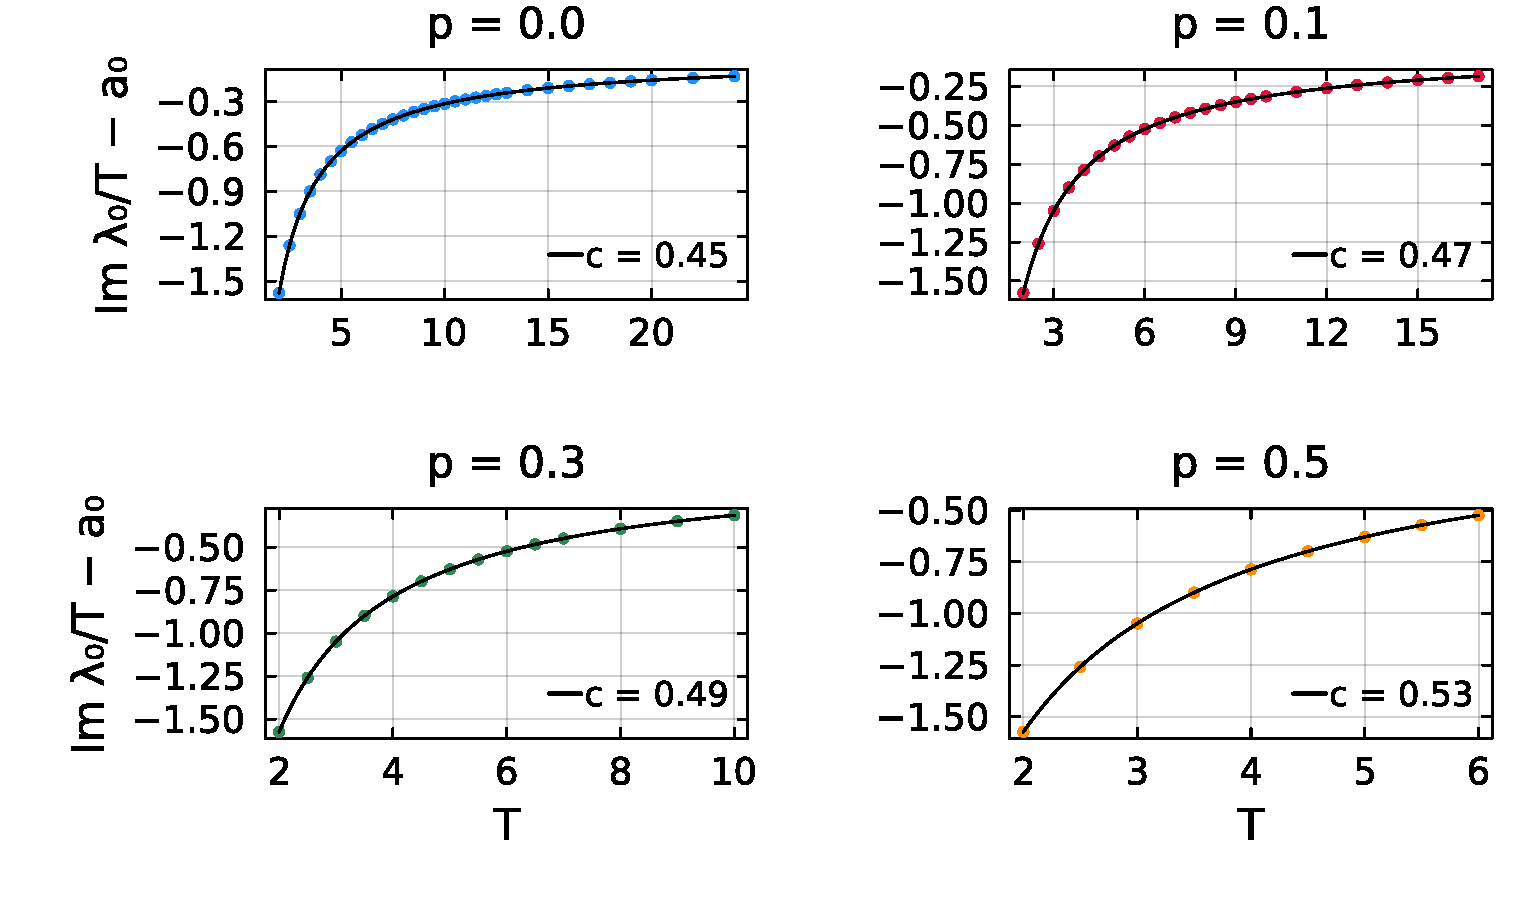
\includegraphics[width=.8\textwidth]{../figures/res_eq3.pdf}

\documentclass[aspectratio=169, 10pt]{beamer}

\usetheme{Madrid}
\usecolortheme{default}
\setbeamertemplate{navigation symbols}{}
\setbeamertemplate{caption}{\insertcaption}

\usepackage{amsmath, amssymb}
\usepackage{graphicx}

\title[Universal properties from dynamics]{Universal properties from quantum many-body dynamics}
\subtitle{Master's thesis defense}
\author[J. G. Márquez Olguín]{Joaquín G. Márquez Olguín \\[1ex] {\small Supervisor: Stefano Carignano (BSC)}}
\institute[]{Barcelona Supercomputing Center}
\date{September 2026}

\begin{document}

% ── title ────────────────────────────────────────────────────────────────────
\begin{frame}
  \titlepage
\end{frame}

\begin{frame}{Outline}
  \tableofcontents
\end{frame}

% ── 1. motivation ────────────────────────────────────────────────────────────
\section{Motivation}

\begin{frame}{Motivation}
  % TODO: universal data from dynamics; why the Loschmidt echo; why non-integrable
\end{frame}

% ── 2. the model ─────────────────────────────────────────────────────────────
\section{The model}

\begin{frame}{The ANNNI-type chain}
  \begin{equation*}
    H = -\sum_i\left[\sigma^z_i\sigma^z_{i+1} + \lambda\,\sigma^x_i
        + p\left(\sigma^z_i\sigma^z_{i+2} + \lambda\,\sigma^x_i\sigma^x_{i+1}\right)\right]
  \end{equation*}
  % TODO: self-dual, critical at lambda = 1, Ising class up to p ~ 1.5
\end{frame}

\begin{frame}{Equilibrium checks}
  % TODO: c(p) from DMRG, sound velocity
  % 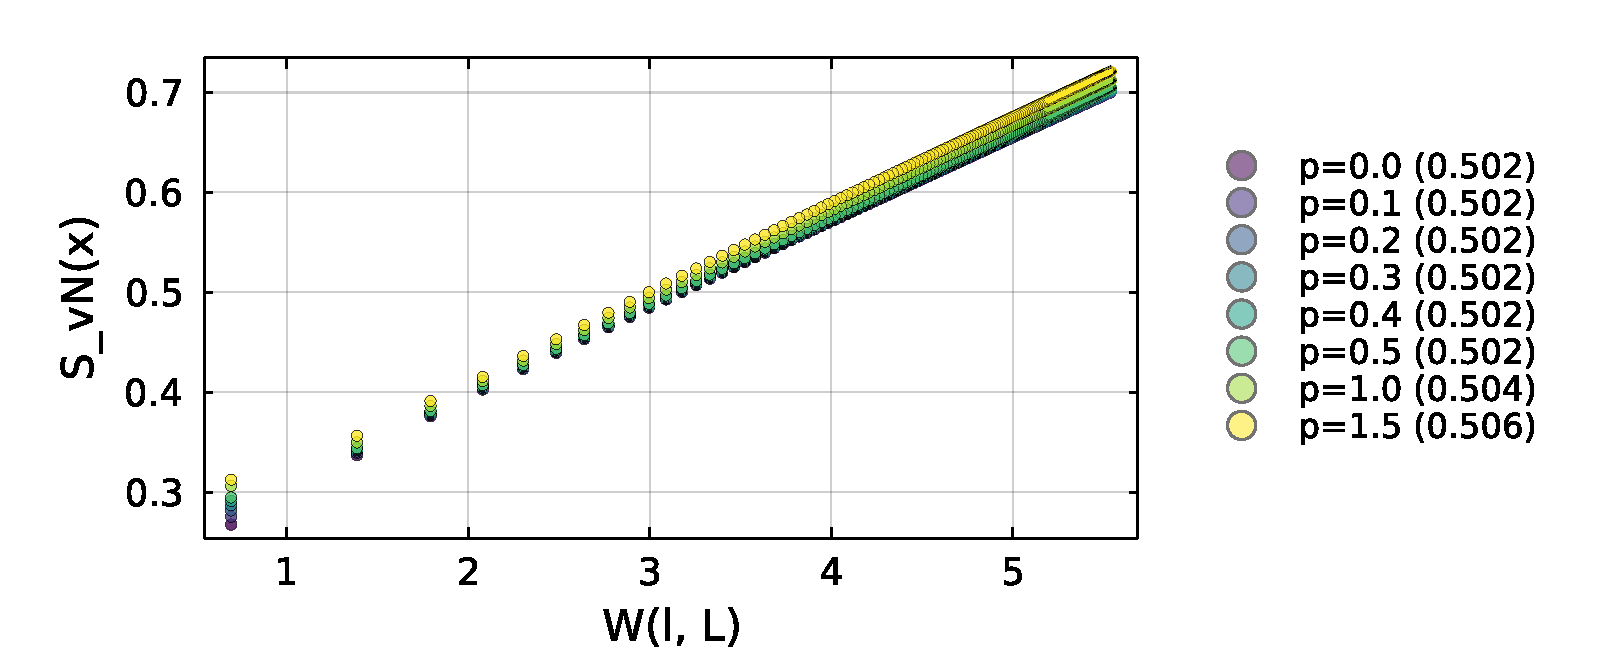
\includegraphics[width=.7\textwidth]{../figures/cft_chord_equilibrium.pdf}
\end{frame}

% ── 3. method ────────────────────────────────────────────────────────────────
\section{Method: transverse contraction}

\begin{frame}{From the echo to a transfer matrix}
  % TODO: echo -> strip partition function -> spatial transfer matrix
\end{frame}

\begin{frame}{The entanglement barrier, and how we sidestep it}
  % TODO: TDVP chi blow-up vs logarithmic temporal entanglement
\end{frame}

\begin{frame}{The corrected transfer-matrix column}
  % TODO: legacy 7 vs corrected 13; validation against Krylov
\end{frame}

\begin{frame}{Validation at the integrable point}
  % TODO: c = 0.4997, x1 = 1/2 and 2, B = -pi
\end{frame}

% ── 4. results ───────────────────────────────────────────────────────────────
\section{Results}

\begin{frame}{The central charge: spectral route}
  % 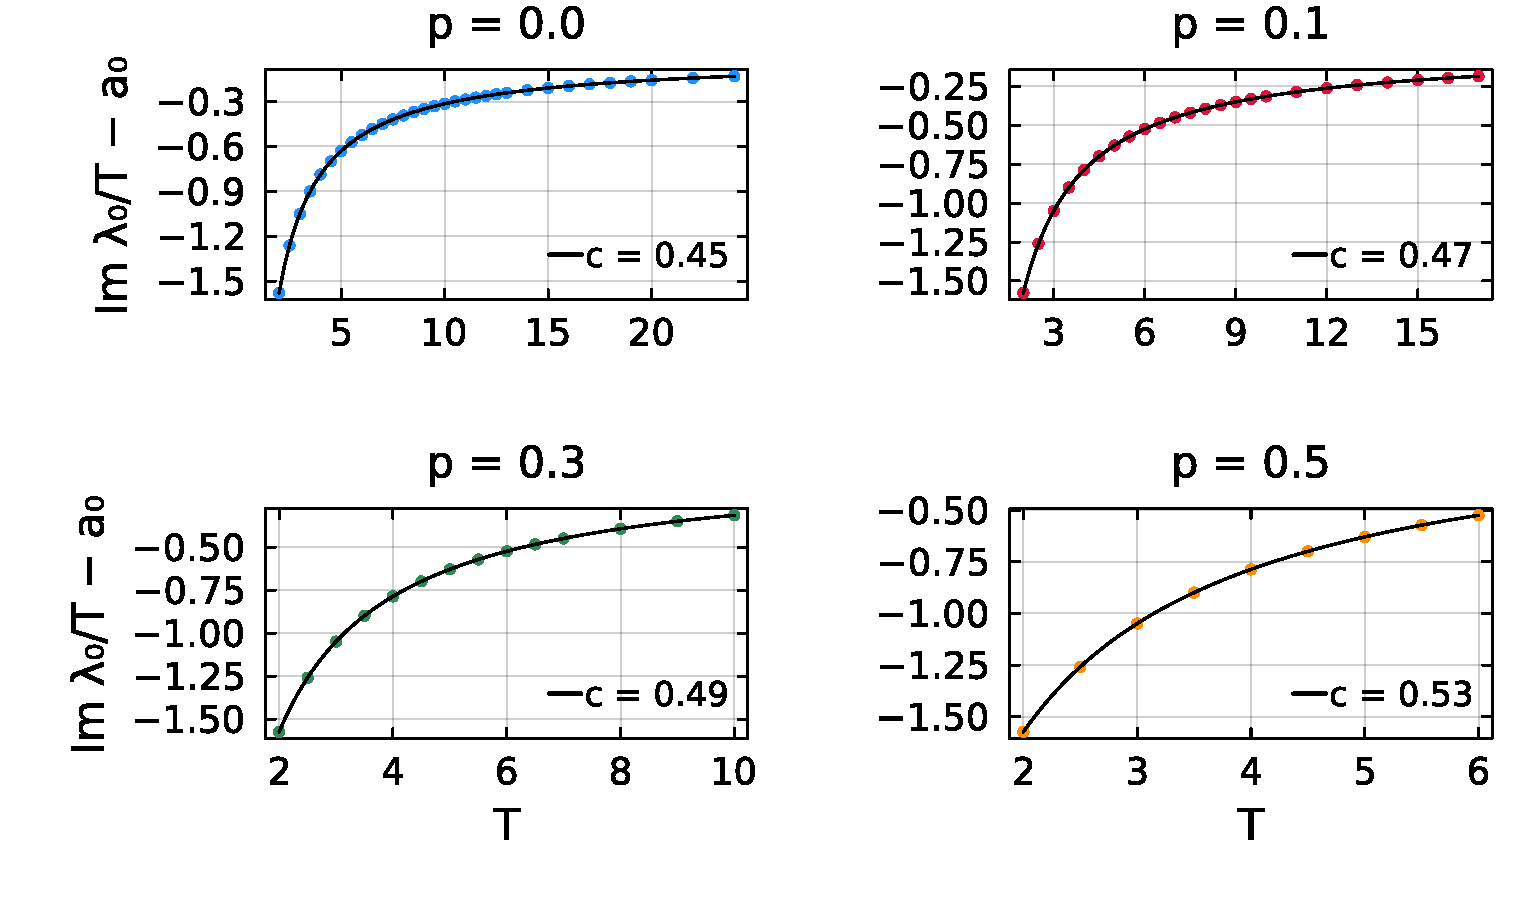
\includegraphics[width=.8\textwidth]{../figures/res_eq3.pdf}
\end{frame}

\begin{frame}{The central charge: entropy route}
  % 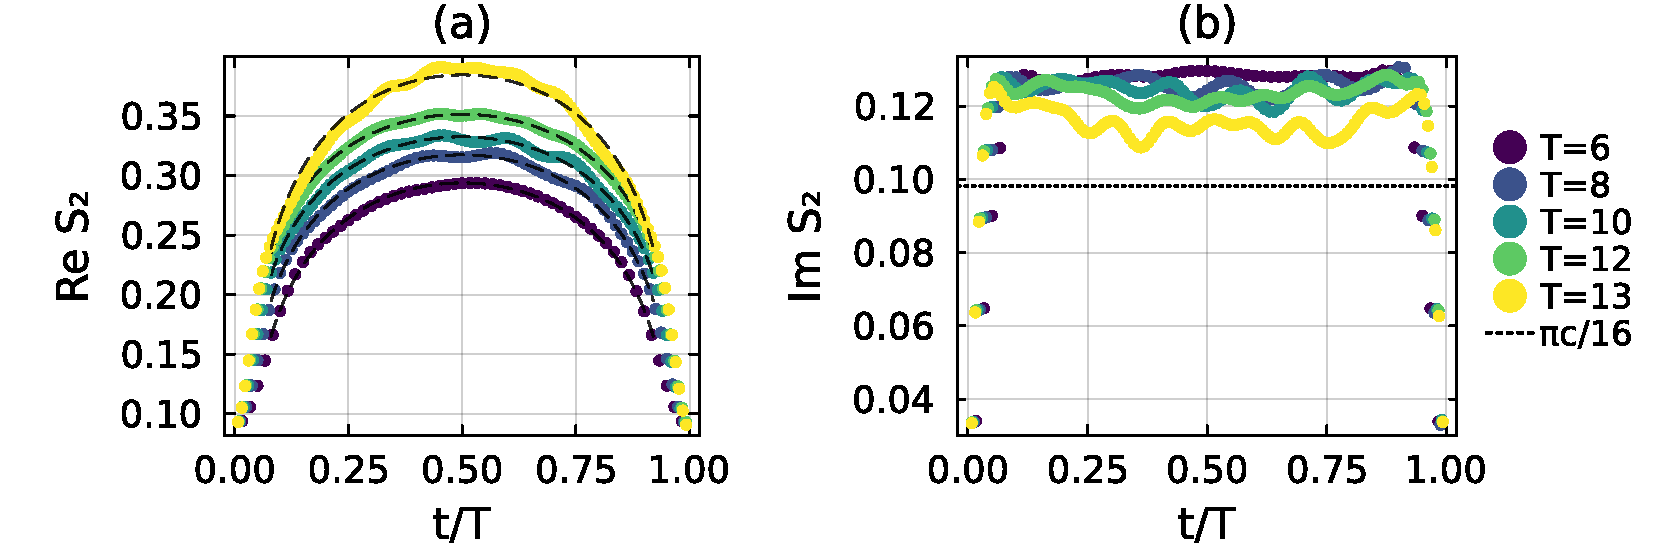
\includegraphics[width=.8\textwidth]{../figures/res_domes.pdf}
\end{frame}

\begin{frame}{The boundary operator spectrum}
  % 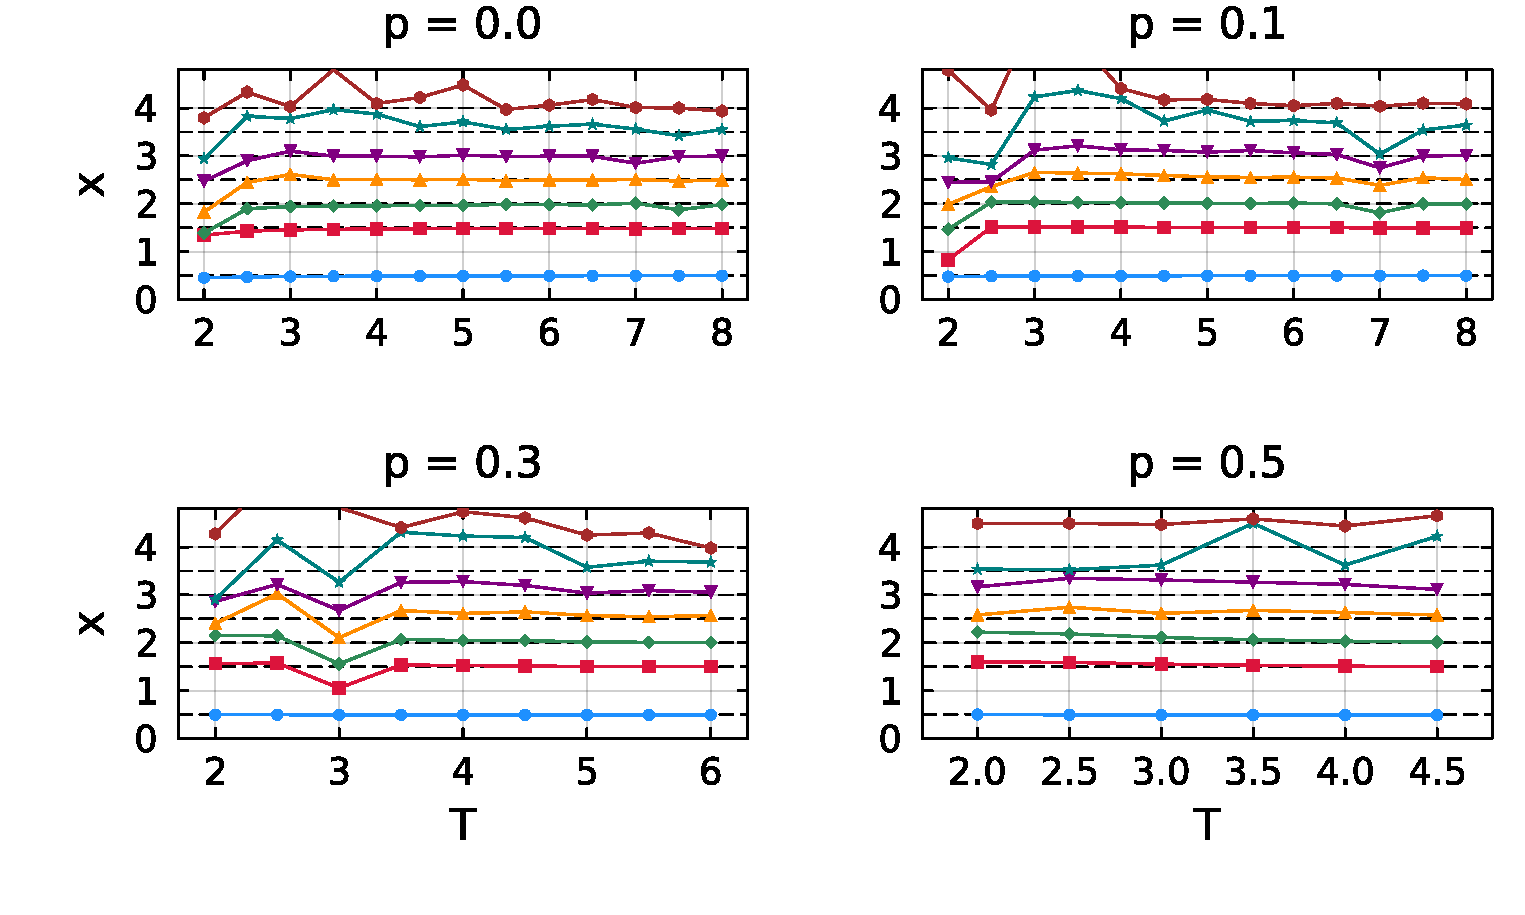
\includegraphics[width=.8\textwidth]{../figures/res_tower.pdf}
\end{frame}

\begin{frame}{The four boundary pairs}
  % 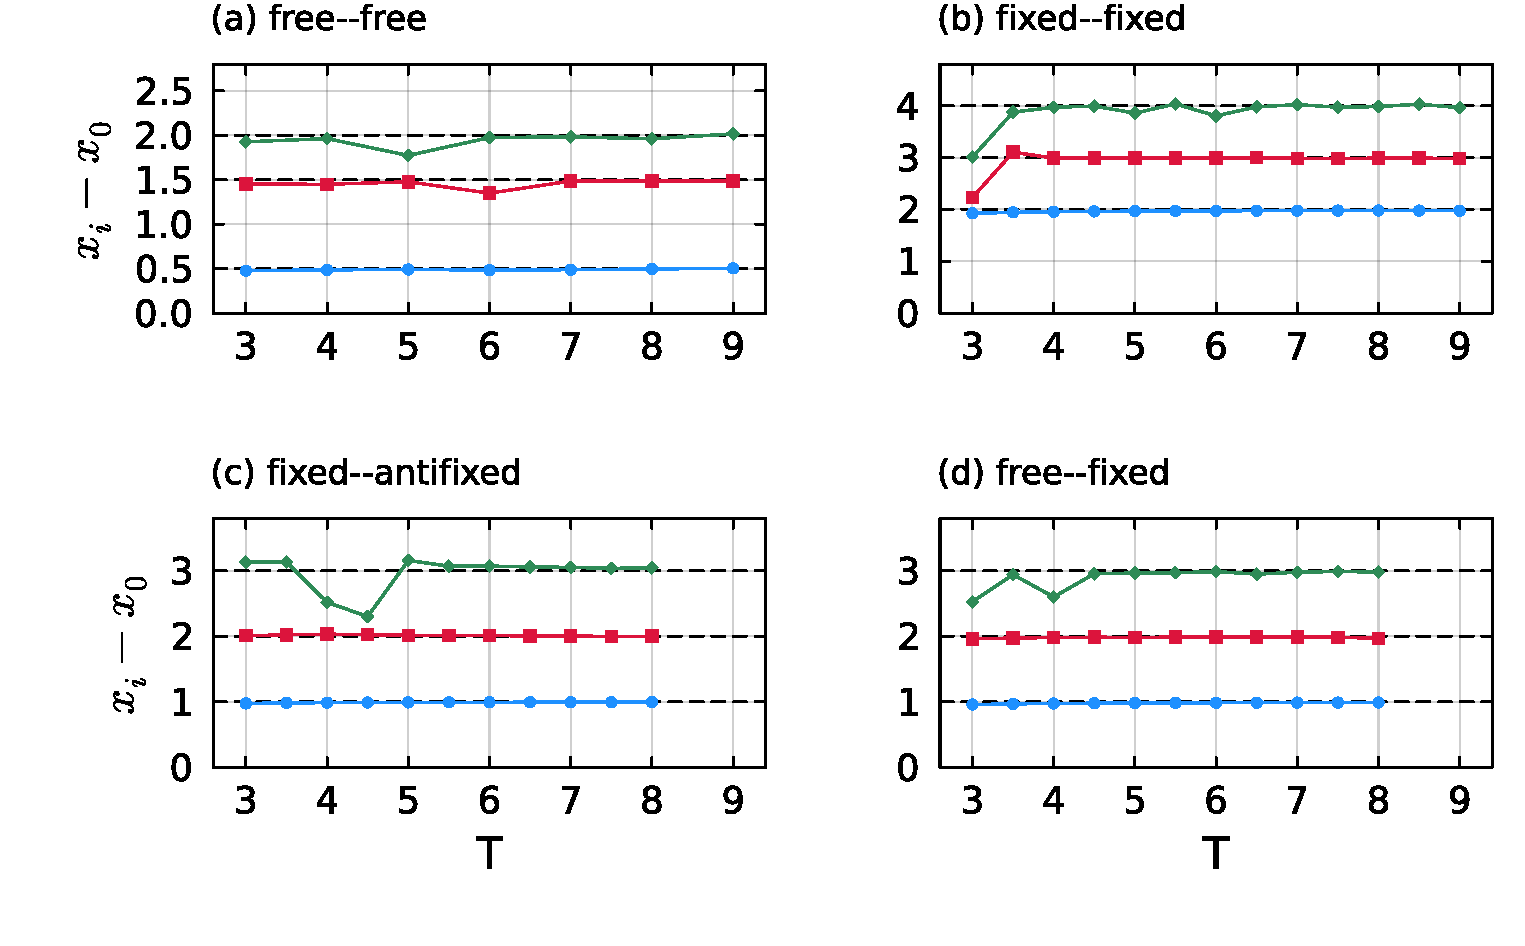
\includegraphics[width=.8\textwidth]{../figures/res_bc_pairs.pdf}
\end{frame}

% ── 5. conclusions ───────────────────────────────────────────────────────────
\section{Conclusions}

\begin{frame}{Conclusions}
  % TODO: the programme survives the loss of integrability; what is measured, what is open
\end{frame}

\begin{frame}
  \centering
  {\Large Thank you}
\end{frame}

% ── backup ───────────────────────────────────────────────────────────────────
\appendix

\begin{frame}{Backup}
  % TODO: controls, failure statistics, beta0 extrapolation, ...
\end{frame}

\end{document}
